\documentclass{article}
\usepackage[landscape, margin=0.25in]{geometry}
\usepackage{graphicx} 
\graphicspath{{/Users/danpost/election_inflation_analysis/output}}
\usepackage{amsmath}
\usepackage{hyperref}
\usepackage{threeparttable}
\usepackage{amsfonts}
\usepackage{listings}
\usepackage{amssymb}
\usepackage{placeins}
\usepackage{subcaption}
\usepackage{float}
%\usepackage{subfigure}
%\usepackage{caption}

\title{Inflation and the 2024 Election}
\author{Daniel Posthumus}

\begin{document}

\maketitle 

\section{Summary}

This is an extension of our write-up trying to match inflation to swings towards Trump. We intuit that the current partisan control of MSAs is one mechanism through which voters perceive the economy, perceptions which they use to make voting decisions. To check this, we incorporate controls related to the current partisan control of MSAs. 

The key takeaway is that it appears voters' reactions to inflation appears structurally different across states, depending on the partisan composition of state government. In particular, it appears that only in states where government was split is there any sort of suggestion of a significant association between intra-MSA variation in inflation and intra-MSA variation in swings towards Trump from 2020-2024.

\section{Results}

The following regression results report the point estimates fitting this linear equation (using cluster-robust errors and OLS):
\begin{gather}
\begin{split}
	\text{SWING}_i = \alpha_0 + \beta_1 (\text{R}_i \times \text{Biden\_RPP\_Change}_i) + \beta_2 (\text{D}_i \times \text{Biden\_RPP\_Change}_i) + \beta_3 (\text{SPLIT}_i \times \text{Biden\_RPP\_Change}_i)  \\
	+ \beta_4 \text{R}_i + \beta_5 \text{D}_i + \beta_6 \text{SPLIT}_i + \beta_7 \text{Biden\_RPP\_Change}_i + \epsilon_i
\end{split}
\end{gather}
where R$_i$, D$_i$, and SPLIT$_i$ are dummy variables referring to whether the state in which a particular MSA, denoted by $i$, is governed by either a unified Republican, unified Democrat, or split government (this data was scraped from Ballotpedia -- shoutout Caleb Brobst for providing the web scraping code).\footnote{Since some MSAs span state lines, in cases where an MSA matched to multiple states, I defaulted to the state higher in population. This was an imperfect solution, I can customize a matching function.}

In the `pres' results, we focus on 2020-2024 swings towards President Trump and for `house' results, we focus on 2020 - 2024 swings towards the Republican House of Representatives candidate. 

\begin{table}[H]
\caption{Regression Results by Category for pres}
\label{tab:regression_results}
\begin{tabular}{lccccccc}
\toprule
category & const & R interaction & D interaction & Split interaction & Split & battleground & battleground interaction \\
\midrule
all items & 2.551 (0.132)*** & -0.153 (0.067)** & -0.224 (0.076)*** & 0.056 (0.156) & 0.320 (0.321) & -1.329 (0.276)*** & -0.096 (0.113) \\
goods & 2.408 (0.123)*** & -0.593 (0.151)*** & -0.371 (0.097)*** & 0.389 (0.268) & 0.872 (0.484)* & -1.537 (0.436)*** & -0.414 (0.236)* \\
housing & 2.534 (0.137)*** & -0.068 (0.015)*** & -0.092 (0.020)*** & -0.090 (0.037)** & 0.492 (0.392) & -1.556 (0.327)*** & 0.039 (0.031) \\
other services & 2.569 (0.130)*** & -0.142 (0.061)** & -0.231 (0.063)*** & 0.175 (0.109) & -0.053 (0.243) & -0.902 (0.205)*** & -0.316 (0.096)*** \\
utilities & 2.554 (0.133)*** & -0.232 (0.052)*** & -0.226 (0.055)*** & -0.336 (0.074)*** & 0.314 (0.422) & -1.351 (0.349)*** & -0.014 (0.062) \\
\bottomrule
\end{tabular}
\end{table}


\begin{table}[H]
\caption{Regression Results by Category for house}
\label{tab:regression_results}
\begin{tabular}{lccccccc}
\toprule
category & const & R interaction & D interaction & Split interaction & R & D & Split \\
\midrule
all items & 2.101 (0.257) & 0.022 (0.198) & -0.007 (0.323) & 0.297 (0.158) & 1.409 (0.572) & 1.400 (0.596) & -0.821 (0.373) \\
goods & 2.394 (0.292) & 0.573 (0.474) & -0.143 (0.340) & 0.738 (0.289) & 1.244 (0.704) & 1.323 (0.698) & -0.842 (0.412) \\
housing & 2.112 (0.285) & -0.045 (0.082) & 0.096 (0.112) & 0.035 (0.036) & 1.596 (0.605) & 1.260 (0.619) & -0.756 (0.395) \\
other services & 2.134 (0.256) & 0.258 (0.135) & -0.119 (0.214) & 0.478 (0.120) & 1.246 (0.545) & 1.498 (0.607) & -0.788 (0.366) \\
utilities & 2.240 (0.240) & 0.566 (0.116) & 0.570 (0.139) & 0.316 (0.106) & 1.168 (0.533) & 1.314 (0.598) & -0.821 (0.374) \\
\bottomrule
\end{tabular}
\end{table}


For context, we can focus on the `goods' category of inflation and visualize the following scatterplots:

\begin{figure}[ht]
\centering
\begin{subfigure}[b]{0.4\textwidth}
    \centering
    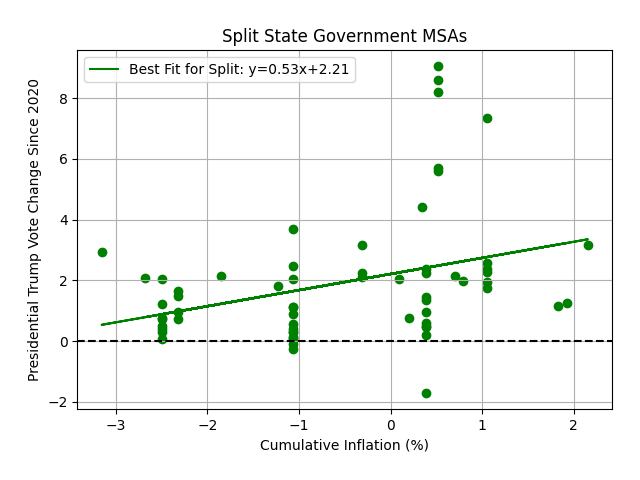
\includegraphics[width=\textwidth]{pres_goods_Split_msa_swing_scatter.png}
\end{subfigure}
\begin{subfigure}[b]{0.4\textwidth}
    \centering
    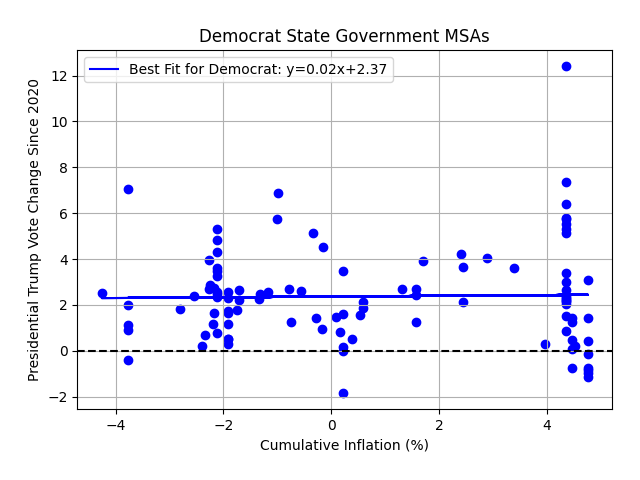
\includegraphics[width=\textwidth]{pres_goods_D_msa_swing_scatter.png}
\end{subfigure}

\begin{subfigure}[b]{0.4\textwidth}
    \centering
    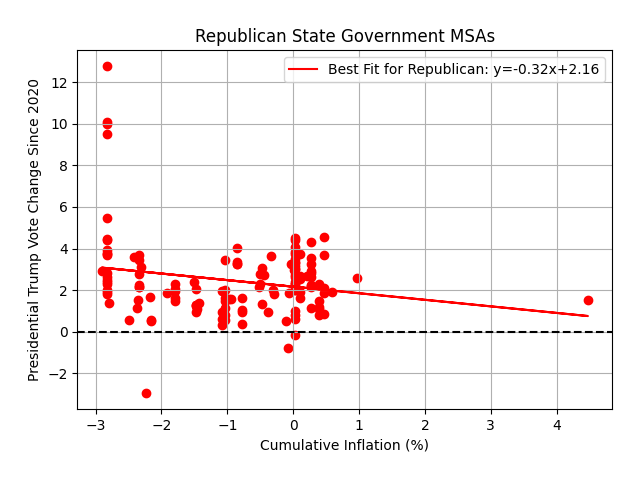
\includegraphics[width=\textwidth]{pres_goods_R_msa_swing_scatter.png}
\end{subfigure}
\caption{Swing Towards President Trump, by State Government Partisan Composition}
\end{figure}

\begin{figure}[ht]
\centering
\begin{subfigure}[b]{0.4\textwidth}
    \centering
    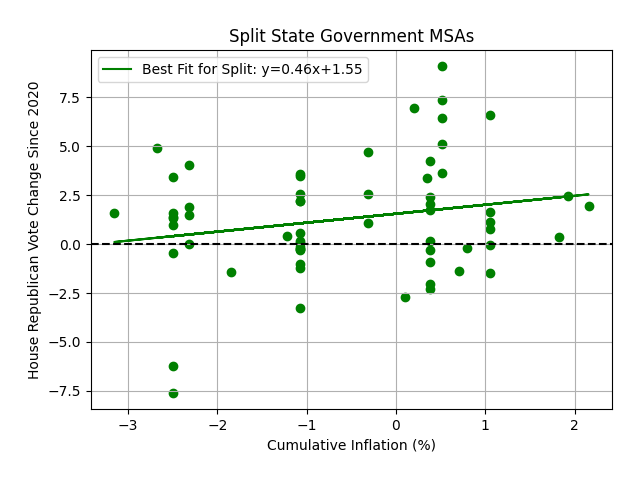
\includegraphics[width=\textwidth]{house_goods_Split_msa_swing_scatter.png}
\end{subfigure}
\begin{subfigure}[b]{0.4\textwidth}
    \centering
    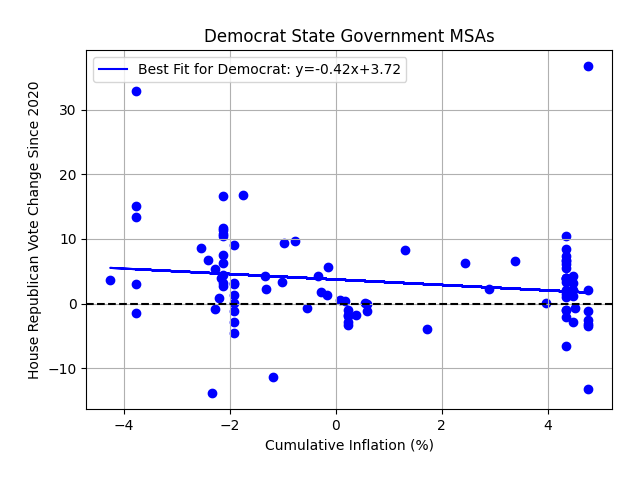
\includegraphics[width=\textwidth]{house_goods_D_msa_swing_scatter.png}
\end{subfigure}

\begin{subfigure}[b]{0.4\textwidth}
    \centering
    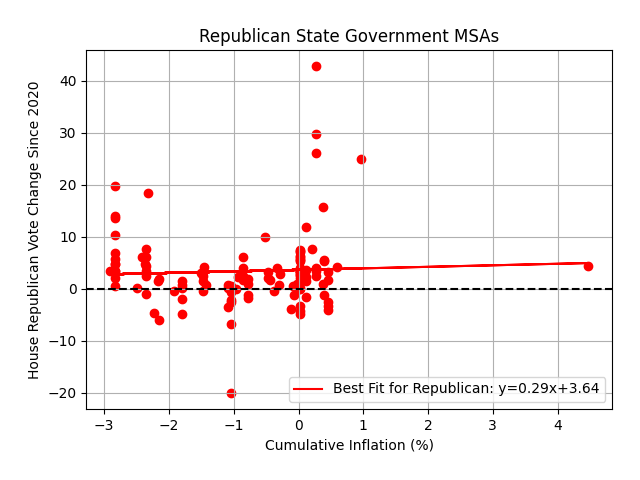
\includegraphics[width=\textwidth]{house_goods_R_msa_swing_scatter.png}
\end{subfigure}
\caption{Swing Towards Republican House Candidates, by State Government Partisan Composition}
\end{figure}

\end{document}